Durante a realização dos testes, o software Htop foi utilizado para monitorar as \textit{threads} criadas nas diferentes execuções do AG em cada uma das arquiteturas. A Figura \ref{figura:res_013} mostra as \textit{threads} criadas pela execução paralela e a Figura \ref{figura:res_014} mostra as \textit{threads} da execução sequencial do AG na Raspberry Pi. As Figuras \ref{figura:res_015} e \ref{figura:res_016} mostram as \textit{threads} criadas, respectivamente, nas execuções paralela e sequencial do AG no \textit{notebook}.
Em ambas as arquiteturas a execução paralela criou 4 \textit{threads}, isso porque o Raspberry Pi possui processador \textit{quad-core} e o \textit{notebook} possui processador \textit{dual-core}, mas devido a tecnologia SMP, o SO reconhece a CPU com quatro núcleos, sendo estes lógicos.

\begin{figure}[htb]  
	\centering
	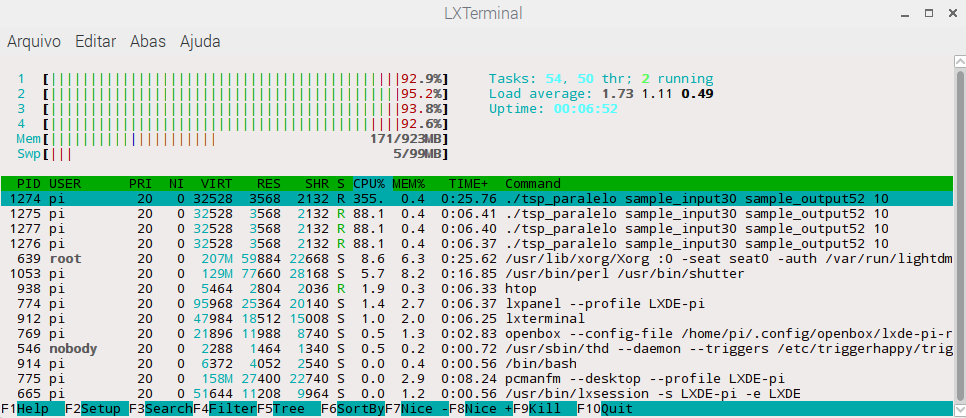
\includegraphics[width=.9\textwidth]{figuras/res_013}
	\caption[Raspberry Pi: AG paralelo]{Raspberry Pi: AG paralelo, em que é possível ver as \textit{threads} criadas durante a execução.}
	\label{figura:res_013}
\end{figure}

\begin{figure}[htb]  
	\centering
	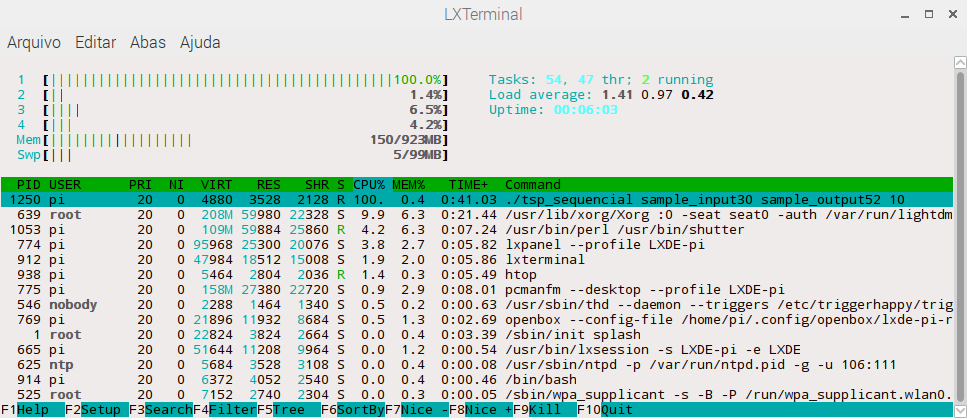
\includegraphics[width=.9\textwidth]{figuras/res_014}
	\caption[Raspberry Pi: AG sequencial]{Raspberry Pi: AG sequencial, em que é possível ver a única \textit{thread} criada durante a execução.}
	\label{figura:res_014}
\end{figure}

\begin{figure}[htb]  
	\centering
	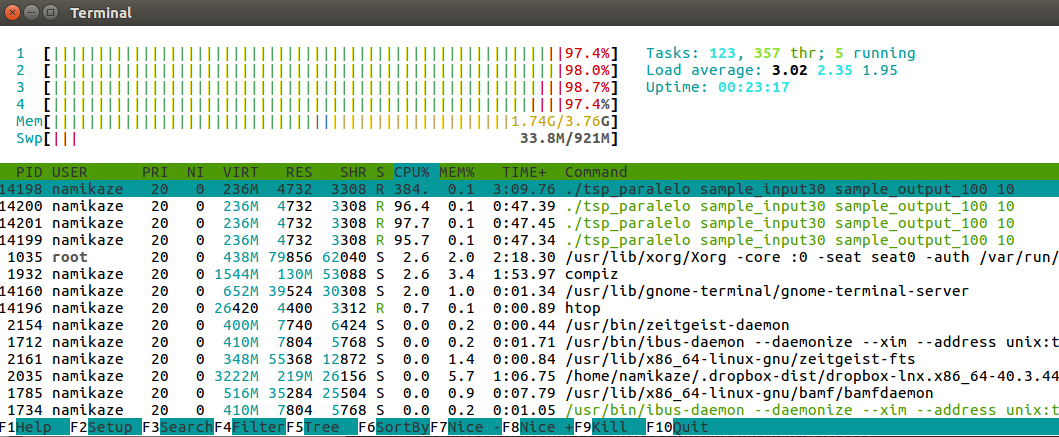
\includegraphics[width=.9\textwidth]{figuras/res_015}
	\caption[\textit{Notebook}:AG paralelo]{\textit{Notebook}:AG paralelo, em que é possível ver as \textit{threads} criadas durante a execução.}
	\label{figura:res_015}
\end{figure}

\begin{figure}[htb]  
	\centering
	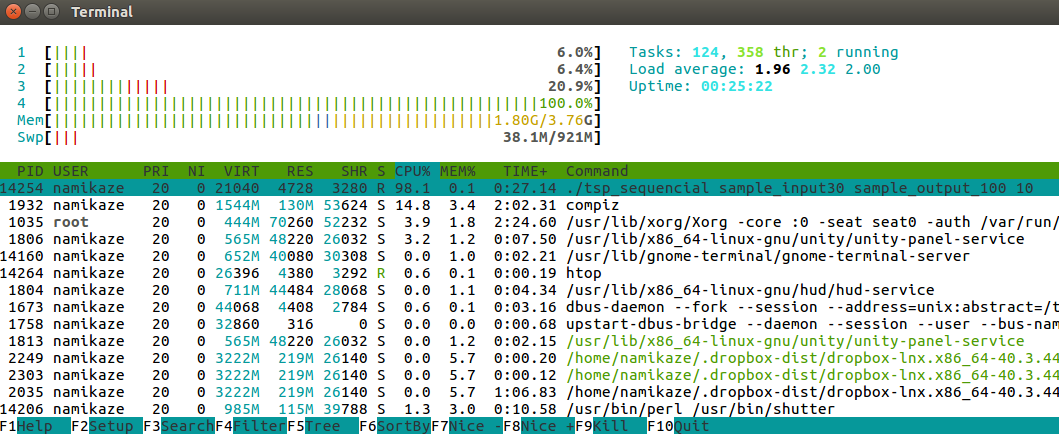
\includegraphics[width=.9\textwidth]{figuras/res_016}
	\caption[\textit{Notebook}: AG sequencia]{\textit{Notebook}: AG sequencial, em que é possível ver a única \textit{thread} criada durante a execução.}
	\label{figura:res_016}
\end{figure}


Após a realização do primeiro teste, que variava o tamanho da entrada, foi possível analisar o comportamento de cada arquitetura tanto no AG paralelo quanto no sequencial. A Figura \ref{figura:res_001} mostra o gráfico obtido do AG sequencial e a  Figura \ref{figura:res_002} mostra o gráfico obtido do AG paralelo executados no \textit{notebook}.

\begin{figure}[htb]  
	\centering
	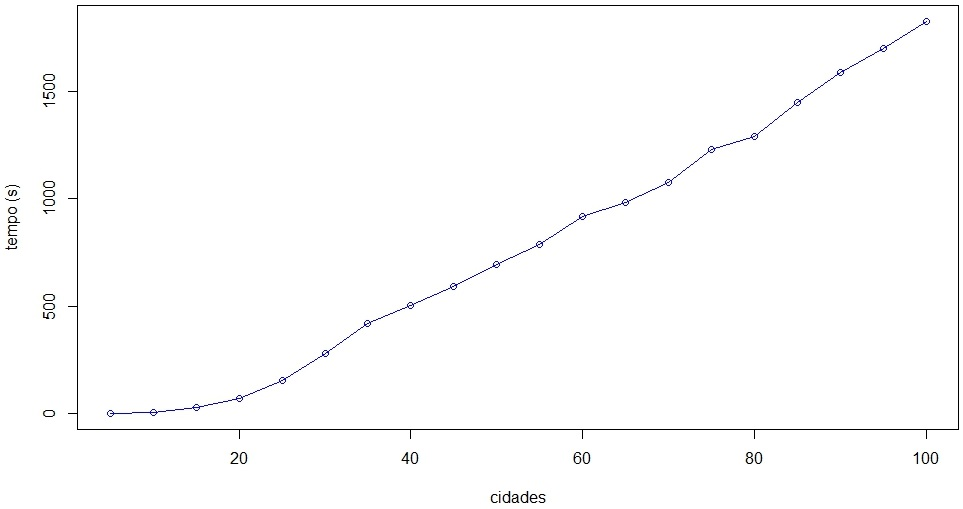
\includegraphics[width=.69\textwidth]{figuras/res_001_20nts}
	\caption[\textit{Notebook}: tempo sequencial]{\textit{Notebook}: Tempo em função da quantidade de cidades no algoritmo sequencial.}
	\label{figura:res_001}
\end{figure}

\begin{figure}[htb]  
	\centering
	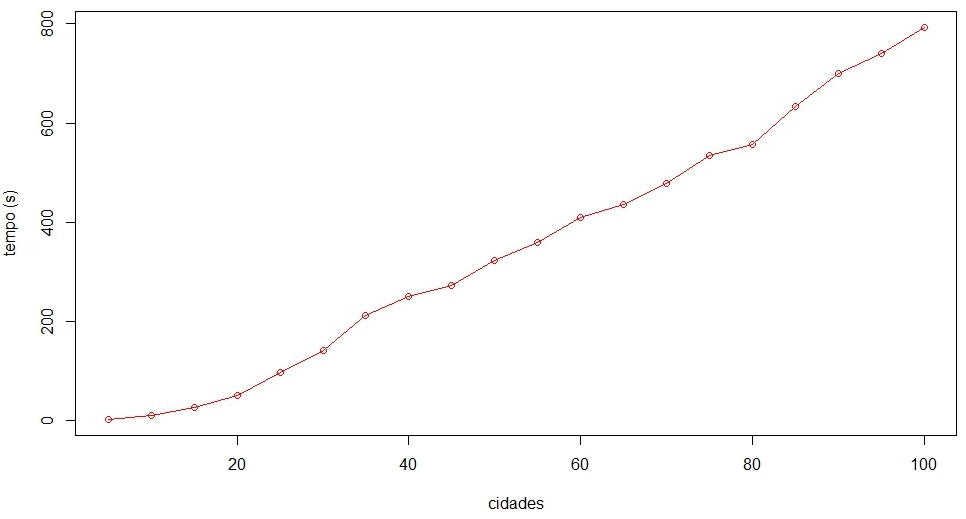
\includegraphics[width=.69\textwidth]{figuras/res_002_20ntp}
	\caption[\textit{Notebook}: tempo paralelo]{\textit{Notebook}: Tempo em função da quantidade de cidades no algoritmo paralelo.}
	\label{figura:res_002}
\end{figure}

As Figuras \ref{figura:res_003} e \ref{figura:res_004} mostram, respectivamente, os gráficos obtidos do AG sequencial e paralelo executados na placa Raspberry Pi.

\begin{figure}[htb]  
	\centering
	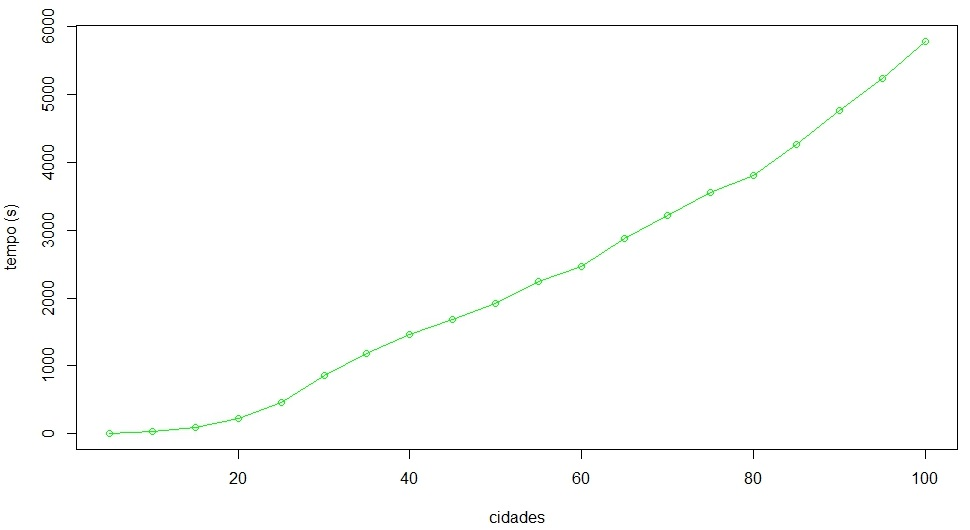
\includegraphics[width=.69\textwidth]{figuras/res_003_20rts}
	\caption[Raspberry Pi: tempo sequencial]{Raspberry Pi: Tempo em função da quantidade de cidades no algoritmo sequencial.}
	\label{figura:res_003}
\end{figure}

\begin{figure}[htb]  
	\centering
	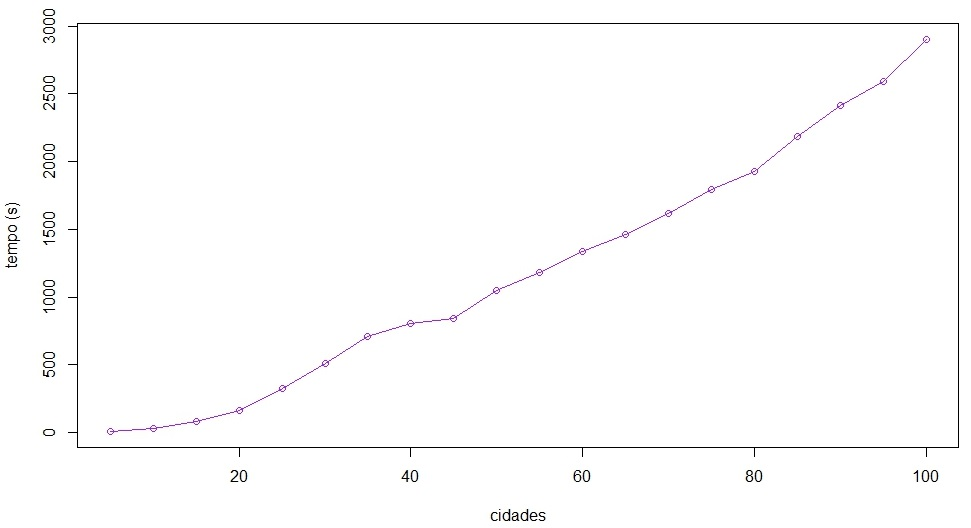
\includegraphics[width=.69\textwidth]{figuras/res_004_20rtp}
	\caption[Raspberry Pi: tempo paralelo]{Raspberry Pi: Tempo em função da quantidade de cidades no algoritmo paralelo.}
	\label{figura:res_004}
\end{figure} 

Observando-se as Figuras \ref{figura:res_001}, \ref{figura:res_002}, \ref{figura:res_003} e \ref{figura:res_004}, pode-se perceber que as arquiteturas apresentam comportamento semelhantes no AG tanto  sequencial quanto no paralelo. O que diferencia é a escala de tempo, já que em cada cenário apresentou faixas de tempo diferentes. É possível notar, também, que o aumento do tempo não apresentou forma exponencial, mas aproximadamente linear. Isso se deve ao uso de heurísticas (na implementação do AG) para resolução de problemas da classe NP-Difícil.

Com base nos tempos adiquiridos, foram calculados o $Sd$ e a $Ef$, que são mostrados na Tabela \ref{tabela:mostragem20}. É possível perceber que o $Sd$ do \textit{notebook} em relação a Raspberry Pi (no AG sequencial e no paralelo) é de aproximadamente 3,3 maior. Ao analisar o $Sd$ do $Tp$ em relação ao $Ts$ do \textit{notebook}, nota-se que o paralelo é quase duas vezes mais rápido que o sequencial. Já no $Sd$ do $Tp$ em relação ao $Ts$ da placa Raspberry Pi, o paralelo é aproximadamente 1,7 vezes mais rápido que o sequencial. As duas arquiteturas apresentaram valores bem próximos de $Ef$, sendo aproximadamente 50\% para o \textit{notebook} e 48\% para a Raspberry Pi.

%j
\begin{table}[htb] \centering
	\caption{Resultados - que incluem a média, mediana e desvio padrão - obtidos a parir do teste realizado com vinte repetições de execução, variando o tamanho das entradas, em cada um dos cenários propostos.} \label{tabela:mostragem20}
	\begin{tabular}{l|ccc}        \hline
		\textbf{Parâmetro analisado} & \textbf{Média} & \textbf{Mediana} & \textbf{Desvio Padrão} \\ \hline \hline		
		\textbf{\textit{Sd Ts} Raspberry/Notebook} 	& 3,2695	& 2,9558 & 1,0925	\\
		\textbf{\textit{Sd Tp} Raspberry/Notebook} 	& 3,3224	& 3,3456 & 0,1667	\\
		\textbf{\textit{Sd} Notebook \textit{Ts/Tp}}		 	& 1,9123	& 2,1792 & 0,5637	\\
		\textbf{\textit{Sd} Raspberry \textit{Ts/Tp}}		 	& 1,7350	& 1,8731 & 0,3314	\\
		\textbf{\textit{Ef} Notebook}			 	& 50,1549	& 54,4800 & 22,9936	\\
		\textbf{\textit{Ef} Raspberry}			 	& 47,9383	& 48,1387 & 21,9332	\\ \hline
	\end{tabular}
\end{table}

As Figuras \ref{figura:res_005} e \ref{figura:res_006} mostram, respectivamente, o comportamento da $Ef$ das arquiteturas conforme a quantidade de cidades no arquivo de entrada. Ao observá-las, fica evidente que a $Ef$ melhora com o aumento da carga de processamento. Isso se deve ao fato de que para pequenas cargas, o custo para divisão das tarefas (alocação e escalonamento de \textit{threads}, por exemplo) reduz a eficiência (aumenta o tempo da execução paralela) das arquiteturas.

\begin{figure}[htb]  
	\centering
	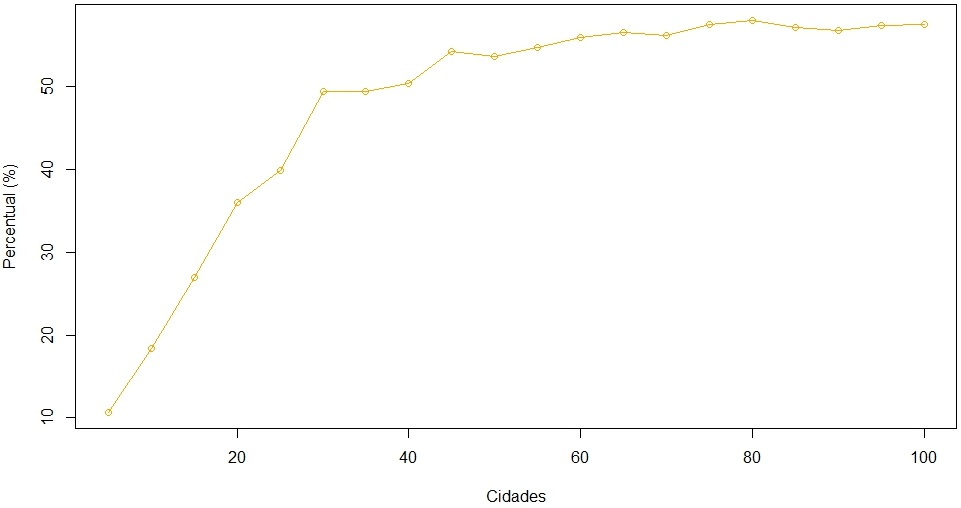
\includegraphics[width=.69\textwidth]{figuras/res_005_20efnt}
	\caption[\textit{Notebook}: eficiência]{\textit{Notebook}: Comportamento da eficiência em função do tamanho das entradas (quantidade de cidades).}
	\label{figura:res_005}
\end{figure} 

\begin{figure}[htb]  
	\centering
	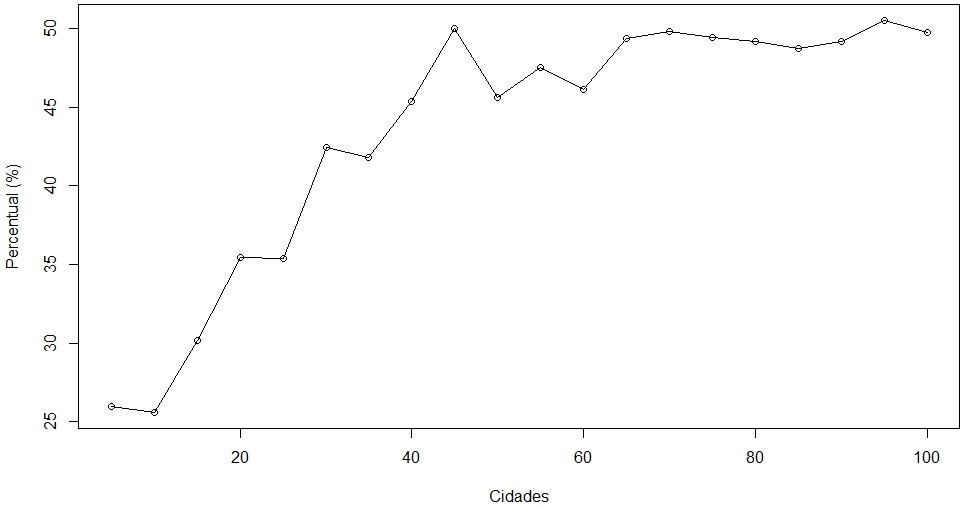
\includegraphics[width=.69\textwidth]{figuras/res_006_20efrp}
	\caption[Raspberry Pi: eficiância]{Raspberry Pi: Comportamente do eficiência em função do tamanho das entradas (quantidade de cidades).}
	\label{figura:res_006}
\end{figure} 

Ao analisar a Figura \ref{figura:res_007}, pode-se perceber a distribuição das medianas dos $Sd_s$ obtidos no primeiro teste, onde é possível notar alguns valores discrepantes (ou \textit{outliers}) no $Sd$ do \textit{notebook} em relação a Raspberry Pi, o que justifica o desvio padrão (Tabela \ref{tabela:mostragem20}) um pouco maior que os demais $Sd_s$ apresentados. Esses valores são resultados de execuções anormais se comparados com a maioria e, mesmo sendo \textit{outliers}, são normais e esperados em sistemas de propósito geral, visto que esses executam outras aplicações ao mesmo tempo, fazendo com que vários fatores interfiram no tempo total de execução.

\begin{figure}[htb]  
	\centering
	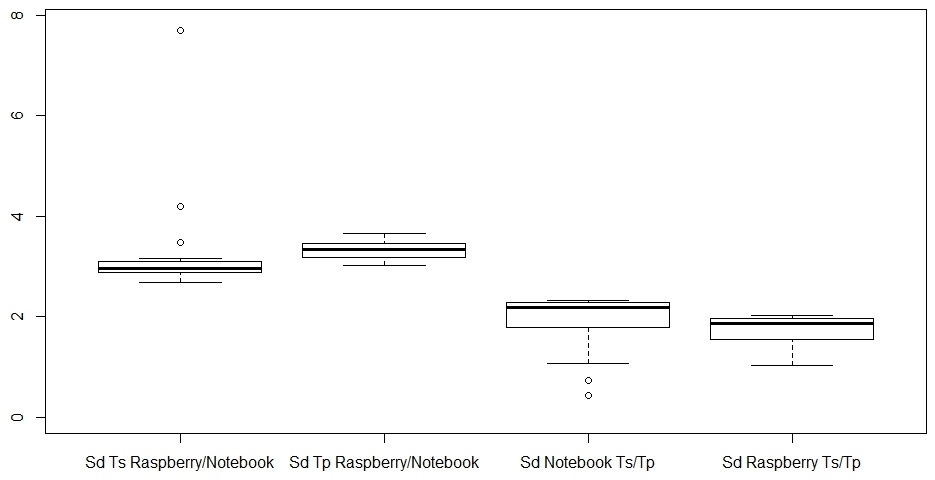
\includegraphics[width=.95\textwidth]{figuras/res_007_20sd}
	\caption[Comparação dos $Sd_s$ obtidos no primeiro teste]{Comparação dos $Sd_s$ obtidos no primeiro teste. O gráfico Boxplot mostra a comparação entre as medianas dos $Sd_s$ obtidos, além de suas variâncias.}
	\label{figura:res_007}
\end{figure} 

No segundo teste, foram repetidas 50 execuções do AG sequencial e paralelo nas duas arquiteturas, sem variar a quantidade de cidades, que foi fixada em 30. Dessa forma, foi possível analisar o comportamento das arquiteturas ao longo do tempo. As Figuras \ref{figura:res_008} e \ref{figura:res_009} apresentam os histogramas de $Ts_s$, $Tp_s$ e $Sd_s$ obtidos no segundo teste.

\begin{figure}[htb]  
	\centering
	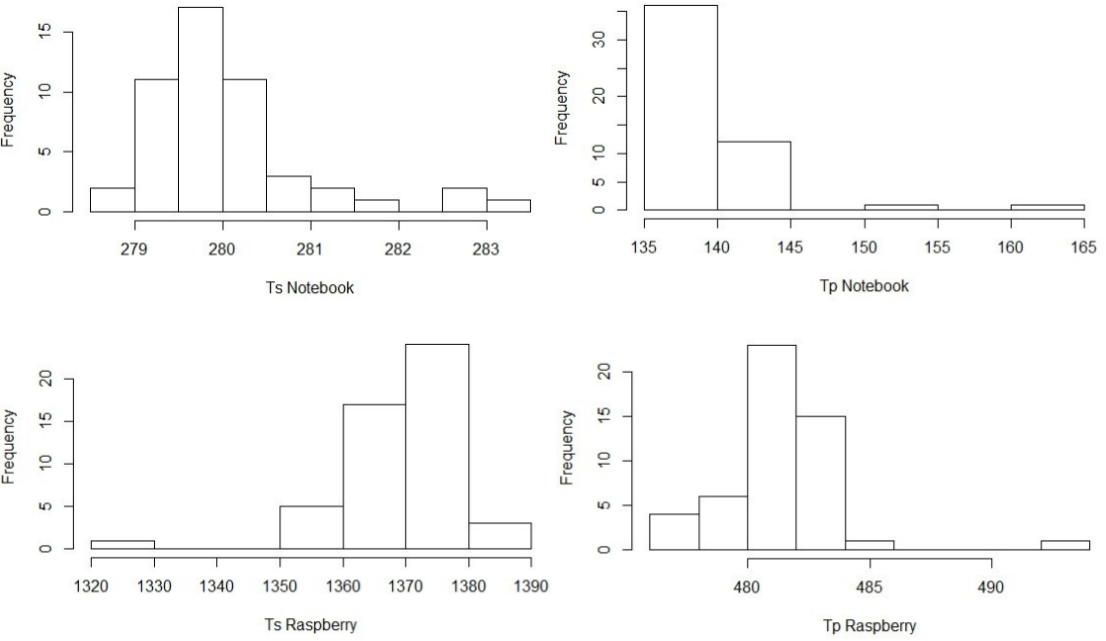
\includegraphics[width=.95\textwidth]{figuras/res_008_50tp}
	\caption[Histogramas dos tempos de execução obtidos]{Histogramas: Os gráficos mostram a frequência das ocorrências dos tempos de execução do AG, em todos os cenários, obtidos no segundo teste.}
	\label{figura:res_008}
\end{figure} 

\begin{figure}[htb]  
	\centering
	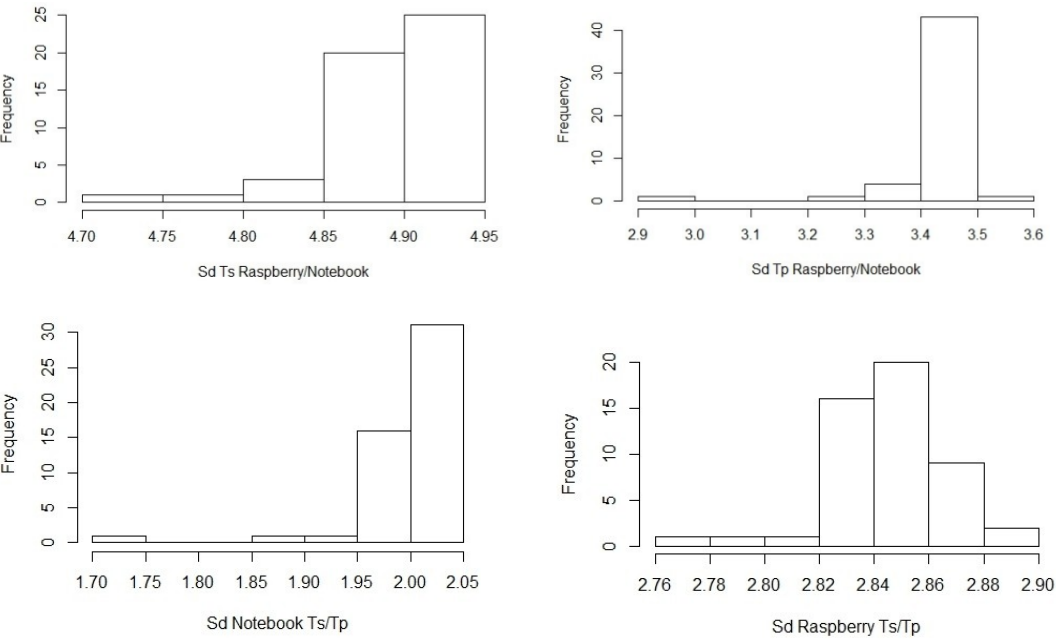
\includegraphics[width=.95\textwidth]{figuras/res_009_50sd}
	\caption[Histogramas dos $Sd_s$ obtidos]{Histogramas: Os gráficos mostram a frequência dos $Sd_s$ ocorridos nos diferentes cenários propostos, obtidos no segundo teste.}
	\label{figura:res_009}
\end{figure} 

Ao analisar a frequência dos tempos de execução, Figura \ref{figura:res_008}, pode-se observar que as arquiteturas apresentaram certa estabilidade nas execuções, visto que ouve pouca variação dos tempos nas faixas de maior frequência. A mesma situação ocorre na Figura \ref{figura:res_009} (frequências altas em faixas pequenas), com os valores de $Sd_s$. A execução sequencial na Raspberry Pi foi a que apresentou maior variabilidade nos tempos. Todos os cenários apresentam alguns valores discrepantes, porém os mesmos são esperados e considerados normais em arquiteturas de propósito geral. A Tabela \ref{tabela:mostragem50} mostra a média, mediana e desvio padrão dos tempos de execução sequenciais e paralelos, $Sd_s$ e $Ef$ das arquiteturas analisadas, que mostram resultados levemente diferentes aos obtidos no primeiro teste: o \textit{notebook} 4,8 vezes mais rápido que a Raspberry Pi no $Ts$ e 3,4 vezes mais rápido no tempo paralelo, o AG paralelo é 1,9 vezes mais rápido que o sequencial no \textit{notebook} e na Raspberry Pi é 2,8 vezes mais rápido.

%j
\begin{table}[htb] \centering
	\caption{Resultados - que incluem a média, mediana e desvio padrão - obtidos a parir do teste realizado com 50 repetições de execuções, com entrada de tamanho fixo, em cada um dos cenários propostos.} \label{tabela:mostragem50}
	\begin{tabular}{l|ccc}        \hline
		\textbf{Parâmetro analisado} & \textbf{Média} & \textbf{Mediana} & \textbf{Desvio Padrão} \\ \hline \hline
		\textbf{\textit{Ts} Notebook}			& 279,7962		  & 279,7430		 & 0,5213	\\
		\textbf{\textit{Ts} Raspberry}			& 1370,545		  & 1373,180		 & 7,0393	\\
		\textbf{\textit{Tp} Notebook}			& 139,5995		  & 139,5775		 & 0,3903	\\
		\textbf{\textit{Tp} Raspberry}			& 481,2862		  & 481,3365		 & 1,5111	\\
		\textbf{\textit{Sd Ts} Raspberry/Notebook} & 4,8897		  & 4,8995			 & 0,0381	\\
		\textbf{\textit{Sd Tp} Raspberry/Notebook} & 3,4266		  & 3,4439			 & 0,0785	\\
		\textbf{\textit{Sd} Notebook \textit{Ts/Tp}}		& 1,9936		  & 2,0032			 & 0,0456	\\
		\textbf{\textit{Sd} Raspberry \textit{Ts/Tp}}		& 2,8449		  & 2,8466			 & 0,0213	\\
		\textbf{\textit{Ef} Notebook}			& 49,8415		  & 50,081			 & 1,1407	\\
		\textbf{\textit{Ef} Raspberry}			& 71,1238		  & 71,165			 & 0,5339	\\ \hline
	\end{tabular}
\end{table}
%j 

As Figuras \ref{figura:res_011} e \ref{figura:res_012} mostram o comportamento, respectivamente, das $Ef_s$ do \textit{notebook} e da Raspberry Pi no decorrer da execuções. Com base nestas imagens e nos valores de $Ef$ apresentados na Tabela \ref{tabela:mostragem50}, nota-se que a Raspberry obteve uma eficiência melhor se comparada ao \textit{notebook}. Isso se deve principalmente as otimizações a nível de SO da placa, por ser um sistema mais limitado em relação ao \textit{notebook}, que permitiram um melhor aproveitamento dos núcleos.

\begin{figure}[htb]  
	\centering
	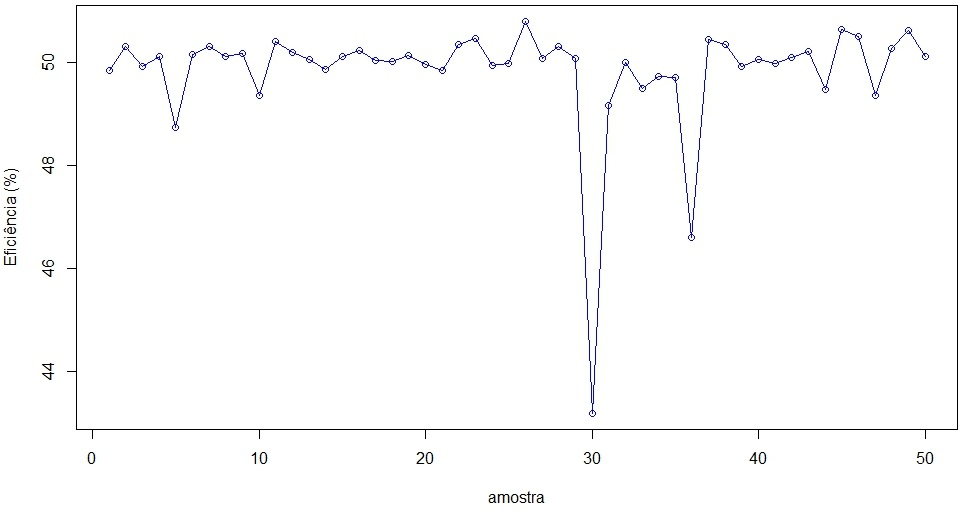
\includegraphics[width=\textwidth]{figuras/res_011_50efnt}
	\caption[\textit{Notebook}: eficiência]{\textit{Notebook}: Comportamento da $Ef$ do \textit{notebook} ao longo das execuções com entradas do mesmo tamanho.}
	\label{figura:res_011}
\end{figure}  

\begin{figure}[htb]  
	\centering
	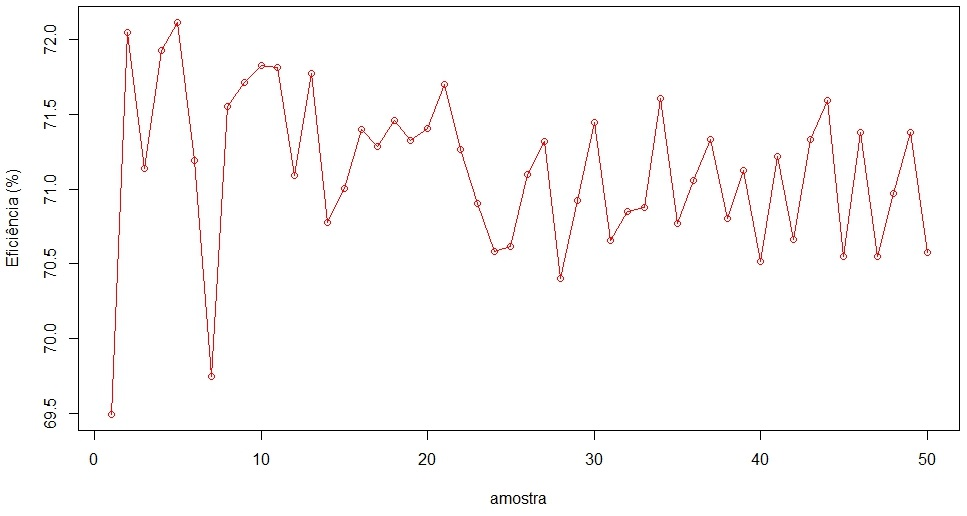
\includegraphics[width=\textwidth]{figuras/res_012_50efrp}
	\caption[Raspberry Pi: eficiência]{Raspberry Pi: Comportamento da $Ef$ da placa Raspberry Pi ao longo das execuções com entradas do mesmo tamanho.}
	\label{figura:res_012}
\end{figure}